\chapter{basic-course-in-mathematics - Formel Samling}

\newpage

\section{Basic}
\subsection{Mängder}
\begin{align*}
  &\quad \text{Naturliga tal: } \mathbb{N} = \{ 1, 2 , 3 ...  \} \\
  &\quad \text{Heltal: }\mathbb{Z} = \{... -2, 1, 0, 1, 2 ...  \} \\
  &\quad \text{Rationella tal: }\mathbb{Q} = \{ \frac{a}{b} | a,b \in \mathbb{Z}, b \\
  &\quad \text{Irrationella tal: }\mathbb{P} = \frac{\mathbb{R}}{\mathbb{Q}}eller \{ x | x \in \mathbb{R}, x \notin \mathbb{Q} \} \\
  &\quad \text{Reella tal: }\mathbb{R} =  \mathbb{P} \cup \mathbb{Q} \\
\end{align*}


\subsection{Potenslagar}
\begin{align*}
  &\quad (\frac{a}{b})^{-3} = (\frac{b}{a})^{3}\\
  &\quad \sqrt{a} = a^{\frac{1}{2}} \\
\end{align*}


\subsection{Logaritmer}
%\begin{align*}
%  &\quad y = a^x \Leftrightarrow \log_a(y) = x  \\
%  &\quad 0<a<1 \text{ och } 1<a \text{ ger olika grafer} \\
%\end{align*}
%
%\begin{tikzpicture}
%\begin{axis}[
%    axis lines = left,
%    xlabel = $x$,
%    ylabel = {$f(x)$},
%]
%%Below the red parabola is defined
%\addplot [
%    domain=-5:5, 
%    samples=100, 
%    color=red,
%]
%{2^x};
%\addlegendentry{$2^x$}
% \addplot [
%    domain=-5:5, 
%    samples=100, 
%    color=black,
%]
%{0.5^x};
%\addlegendentry{$0.5^x$} 
%\end{axis}
%\end{tikzpicture}


\textbf{Logaritmlagar:}\par
Va vaksam över när a<0 då är logarytmen odefinerad. 
\begin{align*}
  &\quad \text{(1): } b = a^x \Leftrightarrow \log_a(b) = x  \text{ för: } a>0, b>0, a \ne 1  \\
  &\quad \text{(2): } \log_a(\frac{b}{c}) = \log_a(b) - \log_a(c) \\
  &\quad \text{(3): } \log_a(b*c) = \log_a(b) + \log_a(c) \\
  &\quad \text{(4): } \log_a(b^d) = d\log_a(b) \\
  &\quad \text{(5): } \log_a(b) = \frac{\log_f(b)}{\log_f(a)} \\
  &\quad \text{(6): } \log_a(a) = 1 \\
  &\quad \text{(7): } \log_a(1) = 0 \\
  &\quad \text{(8): } a^{\log_a(x)} = x \\
  &\quad \text{(9): } \log_{a^c}(b) = \frac{1}{c} \log_a(b) \\
\end{align*}

\subsection{Tillvägagångs sätt}
\begin{equation}
\log_3(x) + \log_x(\frac{1}{27}) = 2
\end{equation}

\subsubsection{Lösning}
\begin{align*}
  &\quad \log_3(x) - 3 \log_x(3) = 2 \\
  &\quad  \log_3(x) - 3 \frac{\log_3(3)}{\log_3(x)} = 2 \\
  &\quad  \log_3(x) - 3 \frac{1}{\log_3(x)} = 2 \\
  &\quad  \log_3(x)^2 - 3 = 2 \log_3(x) \\
  &\quad  y = \log_3(x)^{2} \\
  &\quad  y^2 - 2y- 3 = 0 \\
  &\quad  \text{pq-formeln: } y= 1 \pm \sqrt{4} = 1 \pm 2 \\
  &\quad  \log_3(x) = 3 \Leftrightarrow x = 3^3 = 27 \\
  &\quad  \log_3(x) = -1 \Leftrightarrow x = 3^{-1} = \frac{1}{3} \\
\end{align*}


\subsection{Intervall}
\begin{equation}
[ \, a, b ] \, = \{ x | a \leq x \leq b \}
\end{equation}

\begin{equation}
[ \, a, \infty [ \,
\end{equation}
\begin{equation}
] \, -\infty, \infty [ \,
\end{equation}

\subsection{Tillvägagångs sätt}
\begin{equation}
\frac { 2 } { x - 3 } < \frac { 5 } { x }
\end{equation}


\subsubsection{Lösning}
\begin{align*}
&\quad \frac{ 2 }{ x - 3 } - \frac{ 5 }{ x } < 0 \\
&\quad \frac{(x) 2 }{x (x - 3)} - \frac{ 5 ( x - 3 )}{ x ( x - 3 ) } < 0 \\
&\quad \frac{ 2 x - 5 x - 15 }{ x ( x - 3 ) } < 0 \\
&\quad \frac{ - 3 x - 15 }{ x ( x - 3 ) } < 0 \\
&\quad \frac{ - 3 ( x - 5 ) }{ x ( x - 3 ) } < 0 \\
&\quad  x \neq 0 , x \neq 3 \\
\end{align*}
Värde tabell:
\begin{center}
\begin{tabular}{ |c|c|c|c|c| } 
 \hline
        & x<0   & 0<x<3 & 3<x<5 & 5<x   \\ 
 x-5    & -     & -     & -     & +     \\ 
 -3     & -     & -     & -     & -     \\  
 x      & -     & +     & +     & +     \\ 
 x-3    & -     & -     & +     & +     \\ 
 hela   & +     & -     & +     & -     \\ 
 \hline
\end{tabular}
\end{center}



\section{Komplexa tal}
\begin{align*}
&\quad z = a + bi \\
&\quad \operatorname{Re}(z) = a \\
&\quad \operatorname{Im}(z) = b \\
&\quad \overline{\rm z}= a - b i \\
&\quad | z | = \sqrt{a^ { 2 } + b^ { 2 }} \text{  Där b(Im(z)) är för y-axeln och a(Re(z)) är för x-axeln} \\
&\quad  \\
&\quad \text{Samma räkneregler för reella tal gäller för komplexa tal} \\
\end{align*}


\subsection{Polärform}
\begin{align*}
  &\quad \text{arg}(z) = \alpha + 2\pi * n \\
  &\quad \text{arg(z) är vinkeln mellan a (x-axeln) linjen |z|. n är heltal}  \\
  &\quad \text{Arg}(z) \in ]-\pi, \pi[ \\
    &\quad \text{Arg}(z) \in \text{arg}(z) \\
    &\quad a = |z| \cos{\alpha} \\
    &\quad b = |z| \sin{\alpha} \\
    &\quad z = |z| \cos{\alpha} + i * |z| \sin{\alpha} \\
\end{align*}

\textbf{Polärform:}\par
\begin{equation}
  z = |z|(\cos{\alpha} + i * \sin{\alpha})
\end{equation}

\textbf{Eulers formel:}\par
\begin{equation}
  z = |z|e^{i \alpha}
\end{equation}

\textbf{Sats:}\par
\begin{align*}
  &\quad |z * w| = |z| * |w| \\
  &\quad \text{arg}(z * w) = \text{arg}(z) + \text{arg}(w) \\
  &\quad \text{arg}(\frac{z}{w}) =  \text{arg}(z) - \text{arg}(w)\\
\end{align*}

\newpage

\textbf{De Movre's formel:}\par
\begin{align*}
  &\quad (\cos{(\theta)} + i * \sin{(\theta)})^{n} = \cos{(n*\theta)} + i * \sin{(n*\theta)} \\
\end{align*}


\subsubsection{Binomisk ekvation}
\begin{align*}
  &\quad (\cos{(\theta)} + i * \sin{(\theta)})^{n} = \cos{(n*\theta)} + i * \sin{(n*\theta)} \\
\end{align*}


\subsubsection{Tillvägagångs sätt}
\begin{equation}
  \text{Visa lösningarna i det komplexa tal planet } z^5 = \sqrt{3} + i
\end{equation}

\begin{align*}
  &\quad |\sqrt{3} + i| = \sqrt{\sqrt{3}^2 + 1^2} = \sqrt{4} = 2 \\
  &\quad \left\{ \begin{array} { l } { \sqrt{3} = 2 \cos(\alpha)} \\ { 1 = 2 \sin(\alpha) } \end{array} \right. \\
  &\quad \alpha = \frac{\pi}{6} \\
  &\quad |z|^5(\cos{(5*\theta)} + i * \sin{(5*\theta)}) = 2(\cos{(\frac{\pi}{6})} + i * \sin{(\frac{\pi}{6})}) \\
  &\quad \text{Vilket ger: } \\
  &\quad |z|^5 = 2 \Leftrightarrow |z| = 2^{\frac{1}{5}} \\
  &\quad 5*\theta = \frac{\pi}{6} + 2 \pi n \Leftrightarrow \theta = \frac{\pi}{30} + \frac{2 \pi n}{5} n \in \mathbb{Z} \\
  &\quad \text{I polärform blir det då: } \\
  &\quad z = 2^{\frac{1}{5}} (\cos{\frac{\pi}{30} + \frac{2 \pi n}{5}} + i * \sin{\frac{\pi}{30} + \frac{2 \pi n}{5}}) \\
  &\quad \text{Eulers formel: } z = 2^{\frac{1}{5}} e^{i (\frac{\pi}{30} + \frac{2 \pi n}{5})} \\
  &\quad n = 0,1,2,3,4 \\
  &\quad z_1 = 2^{\frac{1}{5}} e^{i (\frac{\pi}{30})} \\
  &\quad z_2 = 2^{\frac{1}{5}} e^{i (\frac{\pi}{30} + \frac{2 \pi}{5})} \\
  &\quad z_3 = 2^{\frac{1}{5}} e^{i (\frac{\pi}{30} + \frac{4 \pi}{5})} \\
  &\quad z_4 = 2^{\frac{1}{5}} e^{i (\frac{\pi}{30} + \frac{6 \pi}{5})} \\
  &\quad z_5 = 2^{\frac{1}{5}} e^{i (\frac{\pi}{30} + \frac{8 \pi}{5})} \\
\end{align*}

%\begin{figure}
%\begin{tikzpicture}
%[acteur/.style={circle, fill=black,thick, inner sep=2pt, minimum size=0.2cm}
  %\node (a1) at ( 1.3,1.1) [acteur][label=A]{};
%\begin{axis}[
%    xmin=-2.5,
%    xmax=2.5,
%    ymin=-2.5,
%    ymax=2.5,
%    axis equal,
%    axis lines=middle,
%    xlabel=Re($z$),
%    ylabel=Im($z$),
%    disabledatascaling]
%  \fill [opacity=0.3] (0,0) circle [radius=2^(1/5)];
%  \node (a1) at ( 1.3,1.1) [label=z1]{};
%  \filldraw ( 1.3,1.1) circle[radius=1pt];
%  \node (a2) at ( -1.3,1.1) [label=z2]{};
%  \node (a3) at ( -1.3,-1.1) [label=z3]{};
%  \node (a4) at ( 1.3,-1.2) [label=z4]{};
%  \node (a5) at ( 1.8,1.1) [label=z5]{};
%  \draw [-, thick, black] (a1) -- (a2);
%\end{axis}
%\end{tikzpicture}


\newpage
\section{Absolut Belopp}
\subsection{Tillvägagångs sätt}
\begin{equation}
| 2 x - 8 | + | 1 - x | - 2 | x - 3 | = 8 + 3 x
\end{equation}


\subsubsection{lösning}
\begin{align*}
\left( \begin{array} { c } { 2 x - 8 = 0 } \\ { x = 4 } \end{array} \right)
\left( \begin{array} { c } { 1 - x = 0 } \\ { x = 1 } \end{array} \right)
\left( \begin{array} { c } { x - 3 = 0 } \\ { x = 3 } \end{array} \right)
&\quad
&\quad
&\quad
\end{align*}

\begin{align*}
&\quad \text{ I } \left\{ \begin{array} { l } { x \leq 1 } \\ { - ( 2 x - 8 ) + ( 1 - x ) + 2 ( x - 3 ) = 8 + 3 x } \end{array} \right. \\
&\quad \text{ I } \left\{ \begin{array} { l } { x \leq 1 } \\ { - 4 x = 5 } \end{array}  \quad \left\{ \begin{array} { l } { x \leq 1 } \\ { x = - \frac { 5 } { 4 } \text{ lösning}} \end{array} \right. \right. \\
&\quad \text{II } \left\{ \begin{array} { l } { 1 < x \leq 1 } \\ { - ( 2 x - 8 ) - ( 1 - x ) + 2 ( x - 3 ) = 8 + 3 x } \end{array} \right. \\
&\quad \text{II } \left\{ \begin{array} { l } { 1 < x \leq 3 } \\ { - 2 x = 7 } \end{array} \quad \left\{ \begin{array} { l } { 1 < x < 3 } \\ { x = - \frac { 7 } { 2 } \text{ Ej lösning} } \end{array} \right. \right. \\
&\quad \text{III} \left\{ \begin{array} { l } { 3 \leq x < 4 } \\ { - ( 2 x - 8 ) - ( 1 - x ) - 2 ( x - 3 ) = 8 + 3 x } \end{array} \right. \\
&\quad \text{III} \left\{ \begin{array} { l } { 3 \leq x \leq 4 } \\ { - ( 2 x - 8 ) - ( 4 x - 3 ) = 8 + 3 x } \end{array} \quad \left\{ \begin{array} { l } { 3x < 4 } \\ { x = \frac { 5 } { 6 } \text{ Ej lösning} } \end{array} \right. \right. \\
&\quad \text{IV} \left\{ \begin{array} { l } { x \geq 4 } \\ { ( 2 x - 8 ) - ( 1 - x ) - 2 ( x - 3 ) = 8 + 3 x } \end{array} \right. \\
&\quad \text{IV} \left\{ \begin{array} { l } { x \geq 4 } \\ { x = - \frac { 11 } { 2 } \text{ Ej lösning} } \end{array} \right. \\ 
\end{align*}


\newpage

\section{Summor}
\subsection{Aritmetiska summor}
\begin{equation}
s _ { n } = a _ { 1 } + a _ { 2 } + a _ { 3 } + \ldots + a _ { n } = \frac { n \left( a _ { 1 } + a _ { n } \right) } { 2 }
\end{equation}


\subsection{Geometriska summor}
Börjar altid med exponenten 0 och gör om summan så att den passar i följade talföljd:
\begin{equation}
s _ { n } = a + a k + a k ^ { 2 } + \ldots + a k ^ { n - 1 } = \frac { a \left( k ^ { n } - 1 \right) } { k - 1 }
\end{equation}


\subsection{Tillvägagångs sätt}
\begin{equation}
\displaystyle\sum _ { k = n } ^ { 2n } (2^{k} - k)
\end{equation}
\subsubsection{Lösning}
\begin{align*}
  &\quad \text{sätter f = 0 = k -n} \\
  &\quad \displaystyle\sum _ { f = 0 } ^ { n } (2^{f+n} - (f+n)) = 2^{n} * \displaystyle\sum _ { f = 0 } ^ { n } (2^{f}) - \displaystyle\sum _ { f = 0 } ^ { n } (f+n) \\
  &\quad \frac{2^{n} (2^{n+1} -1)}{2-1} - \frac{3n(n+1)}{2} = 2^{2n+1} - 2^{n} - \frac{3n(n+1)}{2}\\
  &\quad  \\
\end{align*}


\newpage

\section{Kombinatorik}
\subsection{Multiplikations principen}
permetationer p(a,b) då ordningen spelar roll. \newline
Antal sätt: (exemplet: antal sätt av måltider 7 företer 5 varmrätter 4 efterätter (7*5*4)
\begin{equation}
n _ { 1 } \cdot n _ { 2 } \cdot \ldots \cdot n _ { m }
\end{equation}


\subsection{Kombinationer}
Kombination c(a,b) då ordningen inte spelar roll. \newline 
Antal sätt: (exemplet: antal del-mängder två element (n = element k = antal element som kan väljas))
\begin{equation}
\left( \begin{array} { l } { n } \\ { k } \end{array} \right) = \frac { n! } { k! (n-k)! }
\end{equation}

\begin{equation}
\left( \begin{array} { l } { n } \\ { k } \end{array} \right) = \frac { n \cdot ( n - 1 ) ( n - 2 ) \cdot \ldots \cdot ( n - 1 ( k - 1 ) ) } { k ! }
\end{equation}


\subsubsection{Pascal triangel}
\begin{center}
\begin{tabular}{>{$}l<{$}|*{7}{c}}
\multicolumn{1}{l}{$n$} &&&&&&&\\\cline{1-1} 
0 &1&&&&&&\\
1 &1&1&&&&&\\
2 &1&2&1&&&&\\
3 &1&3&3&1&&&\\
4 &1&4&6&4&1&&\\
5 &1&5&10&10&5&1&\\
6 &1&6&15&20&15&6&1\\\hline
\multicolumn{1}{l}{} &0&1&2&3&4&5&6\\\cline{2-8}
\multicolumn{1}{l}{} &\multicolumn{7}{c}{$k$}
\end{tabular}
\end{center}


\subsection{Binomial satsen}
\begin{equation}
(a + b)^{n} = \displaystyle\sum _ { k = 0 } ^ { n } \left( \begin{array} { l } { n } \\ { k } \end{array} \right) a ^ {k} b ^ { n - k }
\end{equation}


\newpage

\section{Funktioner och kordinatsystem}
Kom ihåg att när det stor (x-a) förflytas den i x-axeln a steg till höger --> medans (x+a) förflytas den a steg till vänster <-- 
\subsection{Avståndsformeln}
\begin{equation}
d = \sqrt { \left( x _ { 2 } - x _ { 1 } \right) ^ { 2 } + \left( y _ { 2 } - y _ { 1 } \right) ^ { 2 } }
\end{equation}


\subsection{Elipser}
Förenkla till denna formeln:
\begin{equation}
\frac { x ^ { 2 } } { a ^ { 2 } } + \frac { y ^ { 2 } } { b ^ { 2 } } = 1
\end{equation}
Där a är avståndet på x-axeln och b är avståndet på y-axeln


\subsubsection{Hyperbol}
Ser väldigt anerlunda ut från elipser
\begin{equation}
\frac { x ^ { 2 } } { a ^ { 2 } } - \frac { y ^ { 2 } } { b ^ { 2 } } = 1
\end{equation}


\subsubsection{Circkel}
\begin{equation}
\frac { x ^ { 2 } } { a ^ { 2 } } + \frac { y ^ { 2 } } { a ^ { 2 } } = 1
\end{equation}
Där a = r


\newpage

\section{Polynom division}
\subsection{Tillvägagångs sätt}
\begin{equation}
   \text{Man vet att ekvationen} z^4 - 2z^3 - 7z^2 + 26z - 20 = 0 \text{ har roten } z = 2 + i \text{. Lös ekvationen fullständigt.}
\end{equation}
\begin{align*}
  &\quad z = 2 + i \text{ Är en läsning är också konjugatet en lösning enligt faktorsatsen } \overline{\rm z}= a - b i \\
  &\quad z = 2 \pm i \\
  &\quad \text{Vilket betyder att följande går att factorisera ut polynomet} \\
  &\quad (z -(2 + i))(z -(2 - i)) = z^2 - 4z + 5 \\
\end{align*}

\textbf{Långdivition (liggande stolen):}\par
\polylongdiv[style=A]{x^{4}-2x^{3}-7x^{2}+26x-20}{x^{2}-4x+5}%{x ^ { 3 } - 3 x ^ { 2 } - 6 x + 8}{x-1}%{6x^3-2x^2+x+3}{x^2-x+1}

\begin{align*}
  &\quad z^2 + 2z - 4 = 0 \text{ Är också en läsning som tilslut ger följande} \\
  &\quad z = -1 \pm \sqrt{5} \\
  &\quad z = 2 \pm i \\
  &\quad \text{Varge n grads polynom har altid n stycken komplexa lösningar} \\
\end{align*}


\newpage

\section{Trigonometri}
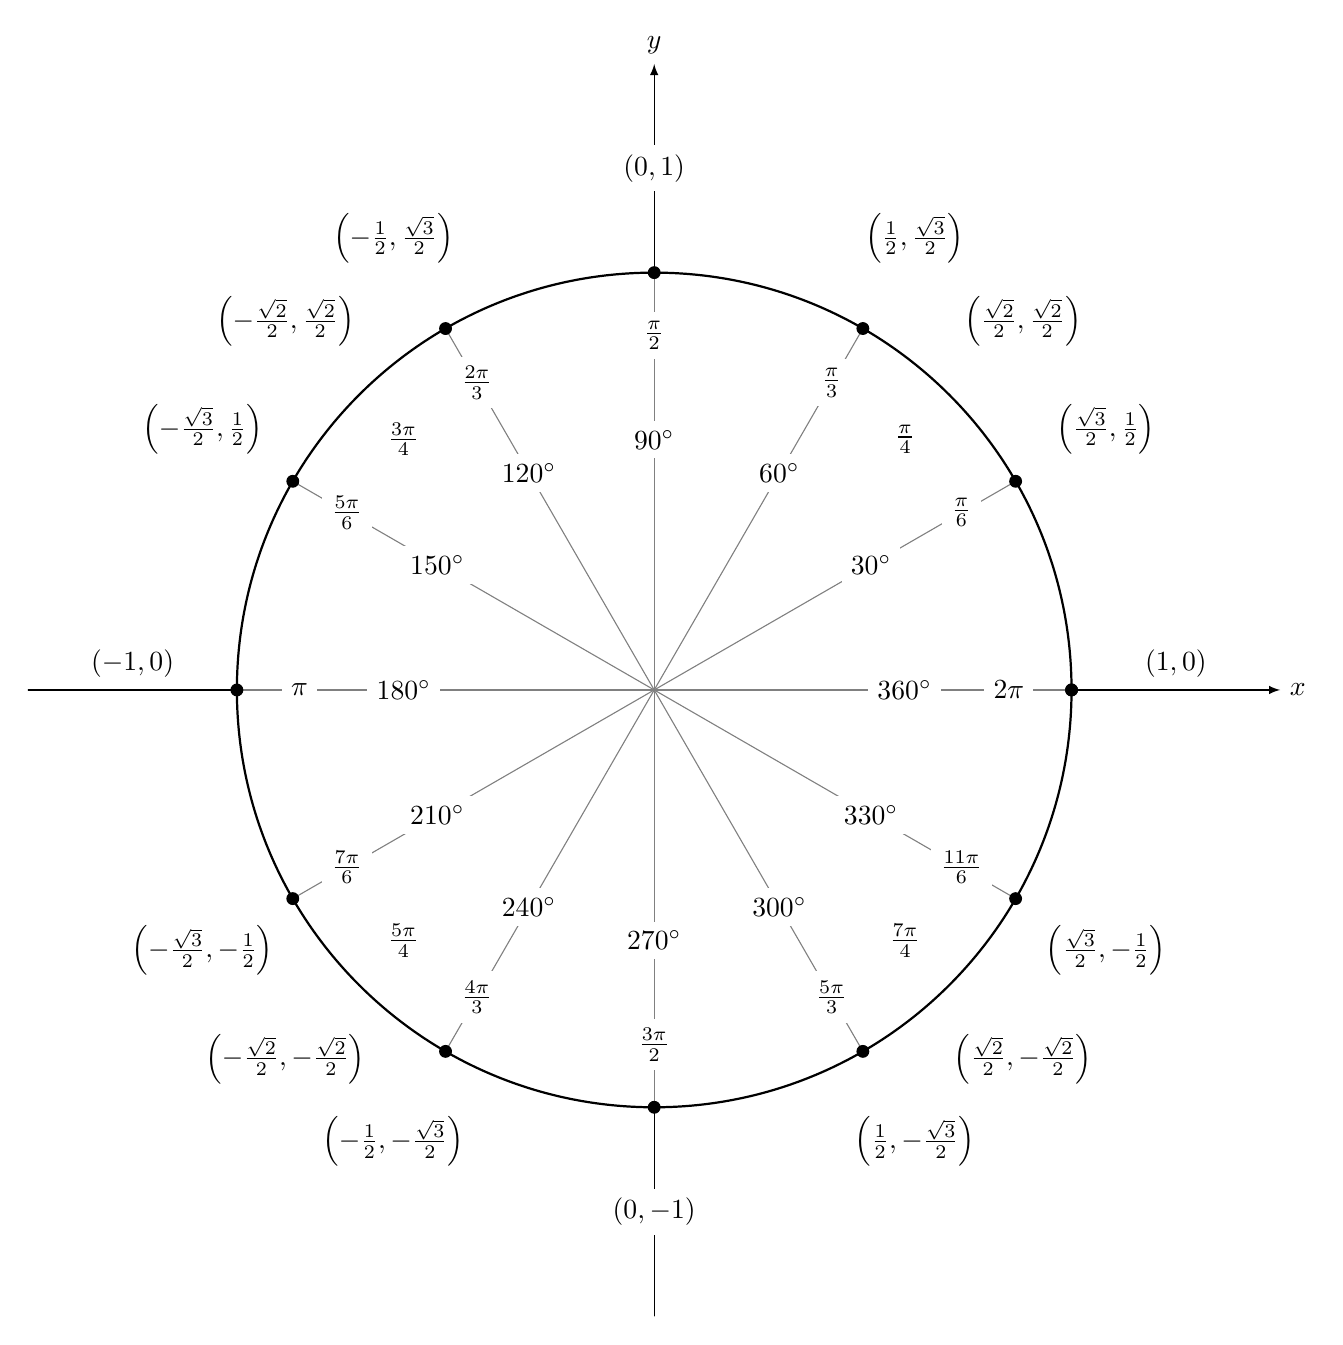
\begin{tikzpicture}[scale=5.3,cap=round,>=latex]
        % draw the coordinates
        \draw[->] (-1.5cm,0cm) -- (1.5cm,0cm) node[right,fill=white] {$x$};
        \draw[->] (0cm,-1.5cm) -- (0cm,1.5cm) node[above,fill=white] {$y$};

        % draw the unit circle
        \draw[thick] (0cm,0cm) circle(1cm);

        \foreach \x in {0,30,...,360} {
                % lines from center to point
                \draw[gray] (0cm,0cm) -- (\x:1cm);
                % dots at each point
                \filldraw[black] (\x:1cm) circle(0.4pt);
                % draw each angle in degrees
                \draw (\x:0.6cm) node[fill=white] {$\x^\circ$};
        }

        % draw each angle in radians
        \foreach \x/\xtext in {
            30/\frac{\pi}{6},
            45/\frac{\pi}{4},
            60/\frac{\pi}{3},
            90/\frac{\pi}{2},
            120/\frac{2\pi}{3},
            135/\frac{3\pi}{4},
            150/\frac{5\pi}{6},
            180/\pi,
            210/\frac{7\pi}{6},
            225/\frac{5\pi}{4},
            240/\frac{4\pi}{3},
            270/\frac{3\pi}{2},
            300/\frac{5\pi}{3},
            315/\frac{7\pi}{4},
            330/\frac{11\pi}{6},
            360/2\pi}
                \draw (\x:0.85cm) node[fill=white] {$\xtext$};

        \foreach \x/\xtext/\y in {
            % the coordinates for the first quadrant
            30/\frac{\sqrt{3}}{2}/\frac{1}{2},
            45/\frac{\sqrt{2}}{2}/\frac{\sqrt{2}}{2},
            60/\frac{1}{2}/\frac{\sqrt{3}}{2},
            % the coordinates for the second quadrant
            150/-\frac{\sqrt{3}}{2}/\frac{1}{2},
            135/-\frac{\sqrt{2}}{2}/\frac{\sqrt{2}}{2},
            120/-\frac{1}{2}/\frac{\sqrt{3}}{2},
            % the coordinates for the third quadrant
            210/-\frac{\sqrt{3}}{2}/-\frac{1}{2},
            225/-\frac{\sqrt{2}}{2}/-\frac{\sqrt{2}}{2},
            240/-\frac{1}{2}/-\frac{\sqrt{3}}{2},
            % the coordinates for the fourth quadrant
            330/\frac{\sqrt{3}}{2}/-\frac{1}{2},
            315/\frac{\sqrt{2}}{2}/-\frac{\sqrt{2}}{2},
            300/\frac{1}{2}/-\frac{\sqrt{3}}{2}}
                \draw (\x:1.25cm) node[fill=white] {$\left(\xtext,\y\right)$};

        % draw the horizontal and vertical coordinates
        % the placement is better this way
        \draw (-1.25cm,0cm) node[above=1pt] {$(-1,0)$}
              (1.25cm,0cm)  node[above=1pt] {$(1,0)$}
              (0cm,-1.25cm) node[fill=white] {$(0,-1)$}
              (0cm,1.25cm)  node[fill=white] {$(0,1)$};
\end{tikzpicture}

\newpage

\textbf{Sats:}\par
\begin{align*}
  &\quad 360^\circ = 2\pi rad \\
  &\quad v_{g} = v_{r} * \frac{180^\circ}{\pi} \\
  &\quad v_{r} = v_{g} * \frac{\pi}{180^\circ} \\
\end{align*}

\textbf{Sats:}\par
\begin{align*}
  &\quad -1 \leq \sin{t} \leq 1 \\
  &\quad -1 \leq \cos{t} \leq 1 \\
\end{align*}

\textbf{Sats:}\par
\begin{align*}
  &\quad \cos{(-t)} = \cos{(t)} \\
  &\quad \sin{(-t)} = -\sin{(t)} \\
  &\quad \tan{(-t)} = \frac{\sin{(-t)}}{\cos{(-t)}} = \frac{-\sin{(t)}}{\cos{(t)}} \\
\end{align*}

\textbf{Additionsformlerna:}\par
\begin{align*}
  &\quad \sin{(\alpha + \beta)} = \sin{(\alpha)}\cos{(\beta)} + \sin{(\beta)}\cos{(\alpha)} \\
  &\quad \sin{(\alpha - \beta)} = \sin{(\alpha)}\cos{(\beta)} - \sin{(\beta)}\cos{(\alpha)} \\
  &\quad \cos{(\alpha + \beta)} = \cos{(\alpha)}\cos{(\beta)} - \sin{(\beta)}\sin{(\alpha)} \\
  &\quad \cos{(\alpha - \beta)} = \cos{(\alpha)}\cos{(\beta)} + \sin{(\beta)}\sin{(\alpha)} \\ 
\end{align*}

\textbf{Trigonometriska ettan:}\par
\begin{align*}
  &\quad (\sin{t})^{2} + (\cos{t})^{2} = 1 \\
  &\quad \sin^{2}{t} + \cos^{2}{t} = 1 \\ 
\end{align*}


\subsection{Tillvägagångs sätt}
\begin{align*}
  \begin{aligned} \cos \frac { \pi } { 12 } & = \cos \left( \frac { \pi } { 3 } - \frac { \pi } { 4 } \right) = \cos \frac { \pi } { 3 } \cos \frac { \pi } { 4 } + \sin \frac { \pi } { 3 } \sin \frac { \pi } { 4 } \\ & = \left( \frac { 1 } { 2 } \right) \left( \frac { 1 } { \sqrt { 2 } } \right) + \left( \frac { \sqrt { 3 } } { 2 } \right) \left( \frac { 1 } { \sqrt { 2 } } \right) = \frac { 1 + \sqrt { 3 } } { 2 \sqrt { 2 } } \end{aligned}
\end{align*}
